\chapter{拉普拉斯矩阵}
\label{chap:graph-laplacian-matrix}

沿用图~\ref{fig:incidence-running-example}中的四点五边图：四条外圈环边为$12,23,34,41$，另有一条对角边$13$。除特别说明外，五条边的权重均取$1$；一般推导考虑至少含一个顶点的有限无向无自环图，边权非负；涉及第二小特征值时另设$n\geq2$。

我们先用一个具体计算引入拉普拉斯矩阵。设顶点$1$的读数为$3$，它的三个邻居$2,3,4$的读数分别为$2,1,0$。将顶点$1$的本点读数分别减去三个邻居的读数，得到$3-2=1$、$3-1=2$、$3-0=3$，三项相加为$6$。这一运算汇总了本点读数相对于所有相邻顶点的偏离总和。

对全图每个顶点同时执行这一运算，就得到顶点空间上的对称线性算子——组合拉普拉斯矩阵$\bm L=\bm D-\bm W$。结合第~\ref{chap:graph-incidence-matrix}章的带符号关联矩阵$\bm B$，这一算子可分解为“沿边取差—乘边权—按顶点汇总”三步复合$\bm L=\bm B\bm C\bm B^\top$，其二次型$\bm x^\top\bm L\bm x=\sum_{\{i,j\}\in E}w_{i,j}(x_i-x_j)^2$直接给出全图各边读数差的加权平方和。

围绕这一核心矩阵，本章按照“矩阵定义—二次型—拉普拉斯谱—生成树计数—按度归一化”的脉络展开：第~\ref{sec:graph-laplacian}节建立加权度、度矩阵以及组合拉普拉斯矩阵$\bm L$的逐点定义与关联矩阵分解；第~\ref{sec:graph-laplacian-energy}节定义拉普拉斯二次型，证明$\bm L$的半正定性等基本性质，阐明二次型与图平滑性及割边权重的结构联系，并简介其在图分割与图信号去噪中的应用。

第~\ref{sec:graph-laplacian-eigenvalues}节研究$\bm L$的拉普拉斯谱，依次讨论特征值、零特征值与连通分量、特征值的上下界、加边单调性以及典型图族的显式谱。

第~\ref{sec:graph-matrix-tree}节将拉普拉斯矩阵的主余子式与除去一个零特征值后的其余特征值乘积应用于生成树计数，证明矩阵树定理、谱计数公式与Cayley公式。

第~\ref{sec:graph-normalized-laplacian}节针对度数不均图上的扩散与划分问题，引入度加权内积、对称归一化拉普拉斯$\mathcal L$与随机游走拉普拉斯$\bm L_{\mathrm{rw}}$，对比两种归一化算子并证明归一化拉普拉斯谱的性质。

\section{组合拉普拉斯}
\label{sec:graph-laplacian}

第~\ref{chap:graph-incidence-matrix}章的关联矩阵$\bm B$把顶点函数映射为沿边差分，又把边上的流量汇总到各顶点。如果将“沿边取差—乘以边权—按顶点汇总”三步复合起来，就得到顶点空间$\mathbb R^n$上的对称线性算子——组合拉普拉斯矩阵$\bm L$。本节依次介绍加权度与度矩阵、组合拉普拉斯矩阵的逐点定义以及它与关联矩阵的分解关系。

\subsection{加权度与度矩阵}
\label{sec:graph-weighted-adjacency}

沿用第~\ref{chap:graph-adjacency-matrix}章的记号。设有限无向无自环图$\mathcal G=(V,E)$有$n$个顶点、$m$条边，加权邻接矩阵$\bm W=(w_{i,j})\in\mathbb R^{n\times n}$在每对相邻顶点$(i,j)$处记录边权$w_{i,j}=w_{j,i}\geq 0$，无边处和对角线处均取零。

给定顶点函数$\bm x\in\mathbb R^n$，矩阵乘积$\bm W\bm x$的第$i$个分量把顶点$i$的所有邻居读数按对应边权加权求和：
\begin{equation}
  (\bm W\bm x)_i=\sum_{j=1}^n w_{i,j}\,x_j.
  \label{eq:graph-weighted-neighbor-sum}
\end{equation}
在图~\ref{fig:incidence-running-example}的四点五边单位权图上取读数$\bm x=(3,2,1,0)^\top$，第一行对顶点$1$的三个邻居$2,3,4$求和，得到$1\cdot2+1\cdot1+1\cdot0=3$；第二行只对顶点$2$的两个邻居$1$和$3$求和，得到$1\cdot3+1\cdot1=4$。如果把所有顶点的读数都取为常值$1$，顶点$1$的输出是$1+1+1=3$，而顶点$2$的输出是$1+1=2$。可见即使各点读数完全相同，$(\bm W\bm x)_i$的数值仍随顶点连接的总边权而不同。

将一个顶点的全部邻边权重相加，就得到该顶点的\term{加权度}（weighted degree），排成对角矩阵即得\emph{度矩阵}（degree matrix）：
\begin{equation}
  d_i=\sum_{j=1}^n w_{i,j}=(\bm W\bm 1)_i,\qquad
  \bm D=\operatorname{diag}(d_1,\ldots,d_n).
  \label{eq:graph-laplacian-weighted-degree}
\end{equation}
在单位权图中，$d_i$就是顶点$i$的邻居个数。若增大某条现有边的权重，只有该边两个端点的加权度随之增加，图的连接结构本身并不改变。由于所有边权非负，加权度$d_i=0$当且仅当顶点$i$关联的所有边权重全为零，即$i$是定义~\ref{def:positive-weight-support}中正权支撑$\mathcal G_+=(V,E_+)$的孤立顶点。

在四点五边算例中，顶点$1,3$各连接三个邻居，顶点$2,4$各连接两个邻居。当五条边均取单位权时，度向量为$\bm d=(3,2,3,2)^\top$；若仅把对角边$13$的权重改为$2$，则两端点$1$和$3$的加权度各增加$1$，度向量变为$(4,2,4,2)^\top$。除特别说明外，后文算例仍取全部边为单位权。

\subsection{组合拉普拉斯的定义}
\label{sec:graph-laplacian-matrix-form}

有了邻居加权和$\bm W\bm x$与度矩阵$\bm D$，就可以把“本点读数相对于各邻居读数的带权偏离总和”写成线性算子。对每条边$\{i,j\}$，用本点读数$x_i$减去邻居读数$x_j$，再乘上边权$w_{i,j}$；把顶点$i$所有邻边的带权差相加，就得到组合拉普拉斯在顶点$i$处的输出。

\begin{definition}[组合拉普拉斯矩阵]
\label{def:graph-combinatorial-laplacian}
设$\bm W$和$\bm D$分别为有限无向非负加权图的加权邻接矩阵和度矩阵。图的\term{组合拉普拉斯}（combinatorial Laplacian）矩阵$\bm L\in\mathbb R^{n\times n}$定义为
\begin{equation}
  (\bm L\bm x)_i=\sum_{j=1}^n w_{i,j}(x_i-x_j),\qquad
  \bm L=\bm D-\bm W.
  \label{eq:graph-combinatorial-laplacian}
\end{equation}
\end{definition}

将式~\eqref{eq:graph-combinatorial-laplacian}第一式按被减数与减数拆开：
\[
  (\bm L\bm x)_i
  =\sum_{j=1}^n w_{i,j}x_i - \sum_{j=1}^n w_{i,j}x_j
  =d_i x_i - (\bm W\bm x)_i.
\]
其中被减数部分$(\bm D\bm x)_i=d_i x_i$收集了本点读数的全部权重系数，减数部分$(\bm W\bm x)_i$则是式~\eqref{eq:graph-weighted-neighbor-sum}的邻居加权和，写成矩阵等式即为$\bm L=\bm D-\bm W$。

当$d_i>0$时，还可从邻域平均的角度理解这一输出。将$d_i$提取出来，式~\eqref{eq:graph-combinatorial-laplacian}可改写为
\[
  (\bm L\bm x)_i = d_i\left(x_i - \sum_{j=1}^n \frac{w_{i,j}}{d_i}x_j\right).
\]
括号内的求和是邻居读数按权重份额$w_{i,j}/d_i$（总和为$1$）计算的加权平均值，因此$(\bm L\bm x)_i$等于加权度$d_i$乘以本点读数高出邻居加权平均值的幅度。

定义~\ref{def:graph-combinatorial-laplacian}是按顶点逐行遍历邻居的写法；若改为按边逐条汇总，就能把$\bm L$与第~\ref{chap:graph-incidence-matrix}章的带符号关联矩阵$\bm B\in\mathbb R^{n\times m}$直接联系起来。固定每条边$e=\{i,j\}$的参考方向$i\to j$，关联矩阵的第$e$列为$\bm b_e=\bm e_i-\bm e_j$。将$\bm L$作用于顶点函数$\bm x$的过程可分解为先后衔接的三步：

第一步是沿边取差。左乘$\bm B^\top$将$n$维顶点函数$\bm x$映射为$m$维沿边差分向量$\bm B^\top\bm x$，其第$e$个分量为
\[
  (\bm B^\top\bm x)_e=\bm b_e^\top\bm x=x_i-x_j.
\]

第二步是按边乘权。左乘边权对角阵$\bm C=\operatorname{diag}(w_{e_1},\ldots,w_{e_m})$，将每条边的差值乘以该边的权重，得到带权边差向量$\bm C\bm B^\top\bm x$，其第$e$个分量为$w_e(x_i-x_j)$。

第三步是按顶点汇总。左乘$\bm B$把每条边的带权差送回它的两个端点：边$e$对应的单列项$w_e\bm b_e(\bm b_e^\top\bm x)$在尾端$i$处加上$w_e(x_i-x_j)$，在头端$j$处加上$-w_e(x_i-x_j)=w_e(x_j-x_i)$。将全部$m$条边的贡献叠加，即得组合拉普拉斯的关联矩阵分解：
\begin{equation}
  \bm L=\sum_{e\in E} w_e\bm b_e\bm b_e^\top
       =\bm B\bm C\bm B^\top.
  \label{eq:graph-laplacian-incidence-factorization}
\end{equation}

在式~\eqref{eq:graph-laplacian-incidence-factorization}的每一项秩一矩阵$w_e\bm b_e\bm b_e^\top$中，列向量$\bm b_e$出现两次。若反转边$e$的参考方向，$\bm b_e$变为$-\bm b_e$，两次负号相互抵消，故$\bm L$完全不依赖各边参考方向的选取。

图~\ref{fig:laplacian-readings-aggregation}在四点单位权图上展示了“沿边取差—乘边权—按顶点汇总”的三步过程。例如边$41$的参考方向为$4\to 1$，沿边差分为$x_4-x_1=0-3=-3$；汇总到头端顶点$1$时乘以$B_{1,41}=-1$得到$-(-3)=+3$，与边$12$送来的$+1$和边$13$送来的$+2$相加，给出$(\bm L\bm x)_1=6$。

\begin{BookInlineFigure}
  \centering
  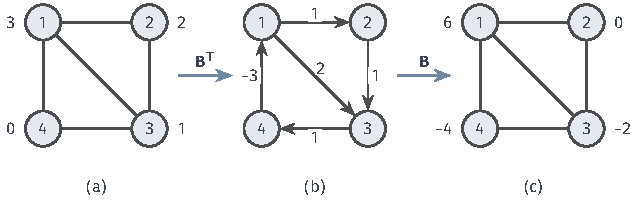
\includegraphics{figures/03-graphs/05-matrices-and-spectra/tikz/laplacian-readings-aggregation.pdf}
  \caption{四点单位权图上计算$\bm L\bm x$的三步分解。（a）顶点旁标注读数$\bm x=(3,2,1,0)^\top$。（b）箭头表示参考方向，边旁数字为沿边差分$\bm B^\top\bm x$（单位权下乘$\bm C$后不变）。（c）左乘$\bm B$汇总回各顶点的输出$\bm L\bm x=(6,0,-2,-4)^\top$。}
  \label{fig:laplacian-readings-aggregation}
\end{BookInlineFigure}

由分解式~\eqref{eq:graph-laplacian-incidence-factorization}立即可见：当所有顶点取同一常数$\bm x=c\bm 1$时，每条边两端读数相等，沿边差分$\bm B^\top(c\bm 1)=\bm 0$，从而$\bm L(c\bm 1)=\bm 0$。无论各顶点的加权度如何分布，全一常向量$\bm 1$始终属于$\bm L$的零空间。

在四点五边单位权算例中，将度向量$\bm d=(3,2,3,2)^\top$填入对角线，并在五条边对应的非对角位置各填$-1$，即得
\[
  \bm L=
  \begin{bmatrix}
  3&-1&-1&-1\\
  -1&2&-1&0\\
  -1&-1&3&-1\\
  -1&0&-1&2
  \end{bmatrix}.
\]
用单位脉冲$\bm e_1=(1,0,0,0)^\top$核对第一列：顶点$1$比三个邻居$2,3,4$各高出$1$，偏离总和为$3$；三个邻居$2,3,4$各自只有一个读数为$1$的邻居，偏离量均为$0-1=-1$，所得$(3,-1,-1,-1)^\top$恰好是$\bm L$的第一列。

\section{拉普拉斯二次型}
\label{sec:graph-laplacian-energy}

上一节给出了组合拉普拉斯矩阵$\bm L=\bm D-\bm W=\bm B\bm C\bm B^\top$及其对顶点函数$\bm x\in\mathbb R^n$的线性作用$\bm x\mapsto\bm L\bm x$。将线性输出$\bm L\bm x$与原向量$\bm x$作内积，就得到实对称矩阵$\bm L$所对应的二次型$\bm x^\top\bm L\bm x$。本节依次介绍拉普拉斯二次型的定义、半正定性等基本代数性质、它与图上顶点读数平滑性及子集割边权重的关系，最后简要介绍它在图分割与图信号处理中的应用。

\subsection{拉普拉斯二次型的定义}
\label{sec:graph-laplacian-quadratic-form}

在线性输出$(\bm L\bm x)_i=\sum_j w_{i,j}(x_i-x_j)$中，同一个顶点与不同邻居的一正一负差值会在求和时相互抵消。例如在三点单位权路径$1\!-\!2\!-\!3$上取$\bm x=(0,1,2)^\top$，中间顶点$2$与左邻$1$相差$+1$、与右邻$3$相差$-1$，相加得到$(\bm L\bm x)_2=0$，仅看该点输出看不出读数正在沿路径递增。

若改为考察二次型$\bm x^\top\bm L\bm x$，利用关联矩阵分解式~\eqref{eq:graph-laplacian-incidence-factorization}，可以把顶点空间上的内积$\bm x^\top(\bm L\bm x)$逐步转写到边空间上。记沿边差分向量为$\bm z=\bm B^\top\bm x\in\mathbb R^m$，其第$e$个分量（对应边$e=\{i,j\}$）为$z_e=x_i-x_j$，则
\[
  \begin{aligned}
    \bm x^\top\bm L\bm x
    &=\bm x^\top(\bm B\bm C\bm B^\top)\bm x\\
    &=(\bm B^\top\bm x)^\top\bm C(\bm B^\top\bm x)\\
    &=\bm z^\top\bm C\bm z\\
    &=\sum_{\{i,j\}\in E}w_{i,j}(x_i-x_j)^2.
  \end{aligned}
\]
若将关于无向边$\{i,j\}\in E$的求和改写为关于全体有序顶点对$(i,j)\in V\times V$的双重求和，每条无向边在$(i,j)$与$(j,i)$处各被计入一次，故须乘以因子$\frac12$。

\begin{definition}[拉普拉斯二次型与沿边变化能量]
\label{def:graph-dirichlet-energy}
设$\mathcal G=(V,E)$为有限无向非负加权图，$\bm L=\bm D-\bm W=\bm B\bm C\bm B^\top$为其组合拉普拉斯矩阵。对任意顶点函数$\bm x\in\mathbb R^n$，称
\begin{equation}
  \bm x^\top\bm L\bm x
  =\lVert\bm C^{1/2}\bm B^\top\bm x\rVert_2^2
  =\sum_{\{i,j\}\in E}w_{i,j}(x_i-x_j)^2
  =\frac12\sum_{i,j=1}^n w_{i,j}(x_i-x_j)^2
  \label{eq:graph-laplacian-energy}
\end{equation}
为$\bm x$的\emph{拉普拉斯二次型}（Laplacian quadratic form），也称为$\bm x$在图上的\term{沿边变化能量}（Dirichlet energy）。
\end{definition}

与逐点线性输出不同，式~\eqref{eq:graph-laplacian-energy}对每条边的两端差值$x_i-x_j$先平方再乘以边权$w_{i,j}$求和，因此不同边上的正负差值不再相互抵消。在刚才的三点路径上，$\bm x=(0,1,2)^\top$的二次型为$(0-1)^2+(1-2)^2=2$，真实反映了读数在两条边上的累积变化。

\subsection{拉普拉斯二次型的性质}
\label{sec:graph-laplacian-quadratic-properties}

由定义式~\eqref{eq:graph-laplacian-energy}中“加权平方和”的结构，可以直接导出组合拉普拉斯矩阵$\bm L$的半正定性以及二次型的平移不变性与边权可加性。

\begin{theorem}[拉普拉斯二次型的性质与半正定性]
\label{prop:graph-laplacian-quadratic-form}
设$\mathcal G=(V,E)$为有限无向非负加权图，组合拉普拉斯矩阵为$\bm L$。则：
\begin{enumerate}
  \item \emph{半正定性}：$\bm L$是实对称半正定矩阵，即对任意$\bm x\in\mathbb R^n$都有$\bm x^\top\bm L\bm x\geq 0$；且$\bm x^\top\bm L\bm x=0$当且仅当在每条正权边$\{i,j\}\in E_+$上都有$x_i=x_j$。
  \item \emph{常数平移不变性}：对任意$\bm x\in\mathbb R^n$和任意实数$c\in\mathbb R$，有
  \[
    (\bm x+c\bm 1)^\top\bm L(\bm x+c\bm 1)=\bm x^\top\bm L\bm x.
  \]
  \item \emph{关于边权的可加性与单调性}：若同一顶点集$V$上的两张非负加权图$\mathcal G_1,\mathcal G_2$按对应边权相加合成图$\mathcal G=\mathcal G_1+\mathcal G_2$，则对任意$\bm x\in\mathbb R^n$有
  \[
    \bm x^\top\bm L(\mathcal G)\bm x
    =\bm x^\top\bm L(\mathcal G_1)\bm x+\bm x^\top\bm L(\mathcal G_2)\bm x
    \geq\bm x^\top\bm L(\mathcal G_1)\bm x.
  \]
\end{enumerate}
\end{theorem}

\begin{proof}
（1）由$\bm W^\top=\bm W$和$\bm D^\top=\bm D$知$\bm L^\top=(\bm D-\bm W)^\top=\bm L$，故$\bm L$是实对称矩阵。在式~\eqref{eq:graph-laplacian-energy}中，由于每条边的权重$w_{i,j}\geq 0$且平方项$(x_i-x_j)^2\geq 0$，各项均非负，故$\bm x^\top\bm L\bm x\geq 0$，即$\bm L$半正定。非负项之和为零当且仅当每一项都为零；对于$w_{i,j}>0$的正权边$\{i,j\}\in E_+$，这等价于$(x_i-x_j)^2=0$，即$x_i=x_j$。

（2）将每个顶点的读数同时加上常数$c$后，任意一条边$\{i,j\}$两端的读数差为$(x_i+c)-(x_j+c)=x_i-x_j$，逐边差值完全不变，代入式~\eqref{eq:graph-laplacian-energy}即知二次型不变（这也与$\bm L\bm 1=\bm 0$一致）。

（3）当边权相加$w_{i,j}=w_{i,j}^{(1)}+w_{i,j}^{(2)}$时，由$\bm L=\sum_{e\in E}w_e\bm b_e\bm b_e^\top$对边权的线性性，有$\bm L(\mathcal G)=\bm L(\mathcal G_1)+\bm L(\mathcal G_2)$。左乘$\bm x^\top$、右乘$\bm x$即得二次型的可加性；再由$\bm x^\top\bm L(\mathcal G_2)\bm x\geq 0$立得不等式。
\end{proof}

\subsection{二次型与图结构}
\label{sec:graph-laplacian-cut-quadratic-form}

式~\eqref{eq:graph-laplacian-energy}将代数二次型$\bm x^\top\bm L\bm x$与图的拓扑连接紧密绑定在一起，主要体现在连续向量的沿边平滑度与离散子集的割边代价两个方面。

对于一般实向量$\bm x\in\mathbb R^n$，$\bm x^\top\bm L\bm x$度量了\emph{顶点函数沿图结构的平滑程度}。在求和式$\sum_{\{i,j\}\in E}w_{i,j}(x_i-x_j)^2$中，每一项都用边权$w_{i,j}$惩罚相邻顶点取值的不一致：如果图中相连的顶点（尤其是边权$w_{i,j}$较大的紧密连接顶点对）拥有相近的读数$x_i\approx x_j$，那么每条边上的$(x_i-x_j)^2$都很小，$\bm x^\top\bm L\bm x$就会非常小；反之，如果相邻顶点的读数剧烈反号或相差悬殊，$\bm x^\top\bm L\bm x$就会很大。

以四点五边单位权图为例，同样取长度为$2$的零和向量作比较。若取$\bm x=(1,1,-1,-1)^\top$，边$12$和边$34$两端读数相同（差为$0$），只有边$23,41,13$跨越正负号（差为$2$），二次型为$3\times 2^2=12$；若改为取$\bm x=(1,-1,1,-1)^\top$，四条外圈环边两端全部正负交替（差均为$2$），二次型增大为$4\times 2^2=16$。

当$\bm x=\bm 1_S$取为某个顶点子集$S\subseteq V$的$0$--$1$指示向量（在$i\in S$处取$1$，在$i\notin S$处取$0$）时，拉普拉斯二次型\emph{精确等于跨子集边界被切断的边的总权重（割边代价）}。对图中任意一条边$\{i,j\}\in E$，若两端点同在$S$内部或同在$V\setminus S$内部，则$\bm 1_S(i)=\bm 1_S(j)$，该边平方差为$0$；只有一端在$S$内、另一端在$V\setminus S$内的跨割边满足$|\bm 1_S(i)-\bm 1_S(j)|=1$，从而贡献其边权$w_{i,j}$：
\begin{equation}
  \bm 1_S^\top\bm L\bm 1_S
  =\sum_{\{i,j\}\in E}w_{i,j}(\bm 1_S(i)-\bm 1_S(j))^2
  =\sum_{i\in S,\,j\in V\setminus S}w_{i,j}
  =c(S,V\setminus S).
  \label{eq:graph-laplacian-cut-energy}
\end{equation}
同理，若用$\pm 1$指示向量$\bm s=2\bm 1_S-\bm 1$（在$S$内取$+1$，在$V\setminus S$内取$-1$）标记二分划分，则每条跨割边两端相差$2$、平方为$4$，从而$\bm s^\top\bm L\bm s=4\,c(S,V\setminus S)$。

图~\ref{fig:laplacian-edge-energy}在四点五边单位权图上展示了两个$0$--$1$指示向量的二次型。图~\ref{fig:laplacian-edge-energy}(a)取$S=\{1,3\}$的指示向量$\bm x=(1,0,1,0)^\top$，对角边$13$两端同在$S$内（差为$0$），四条外圈环边均跨越$S$与$\{2,4\}$（平方差各为$1$），故$\bm x^\top\bm L\bm x=4=c(\{1,3\},\{2,4\})$。图~\ref{fig:laplacian-edge-energy}(b)取单点集$S=\{1\}$的指示向量$\bm e_1=(1,0,0,0)^\top$，被切断的边恰好是与顶点$1$关联的三条边$12,41,13$，故$\bm e_1^\top\bm L\bm e_1=3=d_1$，这与对角元$L_{i,i}=\bm e_i^\top\bm L\bm e_i=d_i$完全一致。

\begin{BookInlineFigure}
  \centering
  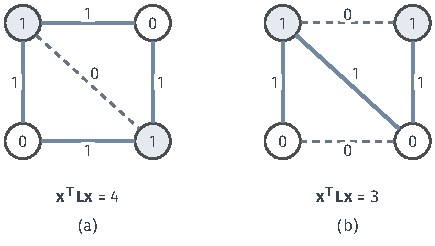
\includegraphics{figures/03-graphs/05-matrices-and-spectra/tikz/laplacian-edge-energy.pdf}
  \caption{四点单位权图上两个$0$--$1$指示向量的拉普拉斯二次型$\bm x^\top\bm L\bm x$。圆内为顶点读数，边旁为该边的平方差$(x_i-x_j)^2$。实线为跨割边（贡献$1$），虚线为同侧边（贡献$0$）。（a）$\bm x=\bm 1_{\{1,3\}}=(1,0,1,0)^\top$的二次型为$4$。（b）$\bm e_1=\bm 1_{\{1\}}=(1,0,0,0)^\top$的二次型为$3=d_1$。}
  \label{fig:laplacian-edge-energy}
\end{BookInlineFigure}

\subsection{在图问题中的应用}
\label{sec:graph-laplacian-quadratic-applications}

得益于“离散指示向量上等于割边代价、连续实向量上度量沿边平滑度”这一双重特性，拉普拉斯二次型在图算法与图数据分析中常作为核心目标函数或正则项出现。

第一类典型应用是\emph{图分割}（graph partitioning）。要把一张图切分为内部连接紧密、跨区连接稀疏的两个子集$S$与$V\setminus S$，就需要最小化跨子集的割边代价$c(S,V\setminus S)=\bm 1_S^\top\bm L\bm 1_S$，同时在子集大小$|S|$或连接体积上施加平衡约束，防止切出孤立小碎片。直接搜索最优离散子集是组合难问题；将离散指示向量松弛为满足正交与长度约束的连续实向量$\bm x\in\mathbb R^n$并最小化二次型$\bm x^\top\bm L\bm x$，离散割问题就转化为对称矩阵的瑞利商极值与特征向量计算问题，这也是第~\ref{chap:spectral-partition}章谱划分方法的出发点。

第二类典型应用是\emph{图信号处理中的去噪与平滑}（graph signal denoising and smoothing）。在传感器网络、社交网络或三维网格上，每个顶点带有一个观测读数$y_i$，排成观测向量$\bm y\in\mathbb R^n$。在采用图平滑先验的模型中，假设待恢复信号在相连顶点之间变化较小，而观测扰动会增加沿边差异；这一假设须与具体数据相符。将拉普拉斯二次型作为图平滑正则项加入最小二乘拟合，可构造如下去噪目标：
\begin{equation}
  \min_{\bm x\in\mathbb R^n}\Bigl\{\lVert\bm x-\bm y\rVert_2^2 + \gamma\,\bm x^\top\bm L\bm x\Bigr\}\qquad(\gamma>0),
  \label{eq:graph-laplacian-denoising}
\end{equation}
其中第一项要求恢复信号$\bm x$贴近观测$\bm y$，第二项以权重$\gamma$惩罚相连顶点之间的数值跳变。

由于$\bm L$半正定，式~\eqref{eq:graph-laplacian-denoising}的目标函数关于$\bm x$严格凸。对$\bm x$求梯度并令其为零，得到线性方程组
\[
  (\bm I+\gamma\bm L)\bm x=\bm y,\qquad
  \bm x=(\bm I+\gamma\bm L)^{-1}\bm y.
\]
该解在拟合观测与降低沿边变化之间作折中；若真实信号含有沿边突变，平滑正则化也可能引入偏差。类似地，若仅在部分边界顶点上已知标签读数，而在其余未知顶点上直接最小化沿边变化能量$\bm x^\top\bm L\bm x$，则得到图上的谐波插值与半监督标签传播；每个正权连通分量都含已知边界顶点时，未知读数唯一确定，其物理对应正是第~\ref{chap:graph-electrical-networks}章电网络中的最小能量原理。

\section{拉普拉斯特征值}
\label{sec:graph-laplacian-eigenvalues}

把一组顶点读数全部乘$2$，每条边的差也乘$2$，平方之后能量变成$4$倍。要比较两组读数在图上变化的方式——而不是单纯因为数值放大而显得能量更高——就需要先把它们缩放到相同的长度。特征向量给出了一组这样的标准方向，特征值告诉我们每个标准方向上的沿边能量。

\subsection{特征向量的变化尺度}
\label{sec:graph-laplacian-frequency}

$\bm L$是实对称矩阵，因此可以取一组标准正交特征向量$\bm u_1,\ldots,\bm u_n$，对应的特征值按$0=\lambda_1\leq\lambda_2\leq\cdots\leq\lambda_n$排列。实对称矩阵的正交谱分解可参考\BookChapterRef{chap:eigen-spectral-decomposition}{卷二"谱分解"章}。

任意顶点读数$\bm x$可以在这组特征基下表示。将$\bm x$投影到每个特征方向上，得到坐标$a_i=\bm u_i^\top\bm x$。这些坐标还原为顶点读数就是
\[
  \bm x=\sum_{i=1}^n a_i\bm u_i.
\]

作用一次拉普拉斯矩阵后，每个方向的坐标从$a_i$变成$\lambda_i a_i$：
\[
  \bm L\bm x=\sum_{i=1}^n\lambda_i a_i\bm u_i.
\]

现在用输入$\bm x$与输出$\bm L\bm x$做内积。由于特征向量两两正交，不同方向的交叉项为零，只有同一方向的坐标相乘。第$i$个方向贡献$a_i\cdot\lambda_i a_i=\lambda_i a_i^2$。类似地，$\bm x$与自身的内积给出各坐标平方之和。这就给出
\begin{equation}
  \bm x^\top\bm L\bm x
  =\sum_{i=1}^n\lambda_i a_i^2,\qquad
  \lVert\bm x\rVert_2^2=\sum_{i=1}^n a_i^2.
  \label{eq:graph-laplacian-spectral-energy}
\end{equation}

当$\bm x$恰好等于某个特征向量$\bm u_i$时，只有第$i$个坐标为$1$，其余全为$0$。此时长度为$1$，能量恰好等于$\lambda_i$。零特征值对应的方向在各连通分量内为常值，沿边没有变化。较小的正特征值对应整图上加权平方差之和较小的读数模式——但这是全图加权累计的结果，并不意味着每条边上的差都比其他方向小。

下面在四点图上逐个核验。先取
\[
  \bm x=(0,1,0,-1)^\top.
\]
顶点$1$的三个邻居$2,3,4$读数分别为$1,0,-1$，差值为$-1,0,1$，加起来为$0$。类似地，顶点$3$的输出也为$0$。顶点$2$的两个邻居$1$和$3$都是$0$，差值都等于自己，输出$2$。顶点$4$的两个邻居也都是$0$，输出$-2$。因此$\bm L\bm x=(0,2,0,-2)^\top=2\bm x$，这是特征值$2$的方向。

将此向量归一化为$\bm x/\sqrt2=(0,1/\sqrt2,0,-1/\sqrt2)^\top$。四条环边中，$12$和$41$的差平方为$1/2$，$23$和$34$也是$1/2$，共贡献$4\cdot(1/2)=2$。对角边$13$两端都是$0$，没有贡献。单位向量的总能量为$2$，确实等于特征值。

换成$\bm x=(1,0,-1,0)^\top$。顶点$1$的两个环邻居$2$和$4$各差$1$，对角邻居$3$差$2$，总和$1+2+1=4$。顶点$3$对称地得到$-4$。顶点$2$和$4$的两个邻居一正一负，恰好相消。因此$\bm L\bm x=(4,0,-4,0)^\top=4\bm x$，特征值为$4$。

最后取$\bm x=(1,-1,1,-1)^\top$。四条环边每对相邻顶点取值相差$2$，差平方为$4$。对角边$13$两端都是$1$，差为零。每个顶点的两个环邻居各贡献$2$，对角邻居（如果有的话）贡献$0$或$2$。以顶点$1$为例，邻居$2,3,4$的差值为$2,-2,2$，之和为$4\cdot1$，于是$\bm L\bm x=4\bm x$，特征值同样为$4$。

这三个非零特征方向加上常向量$(1,1,1,1)^\top$，构成四维空间的一组正交基。四点算例的完整拉普拉斯谱是$0,2,4,4$。特征值$4$出现两次，对应的两个特征向量$(1,0,-1,0)^\top$和$(1,-1,1,-1)^\top$描绘了不同的变化方式，但单位长度下的总能量相同。

图~\ref{fig:laplacian-four-modes}把四个单位特征向量画在同一张图上。比较后面两个方向：$(1,0,-1,0)^\top$在对角边上两端读数不同，$(1,-1,1,-1)^\top$在对角边上两端相同。但加上四条环边的贡献后，两者的总能量都等于$4$。

\begin{BookInlineFigure}
  \centering
  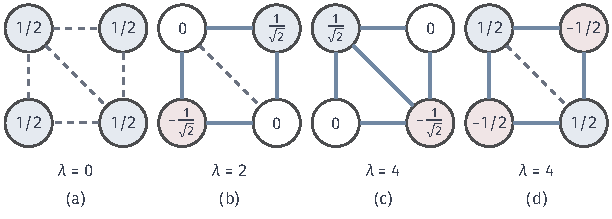
\includegraphics{figures/03-graphs/05-matrices-and-spectra/tikz/laplacian-four-modes.pdf}
  \caption{四点单位权图的四个单位特征向量。圆内为该点的坐标，浅蓝、浅红和白色分别表示正、负和零。两端读数不同的边画成实线，读数相等的边画成虚线。每幅图下的特征值就是沿边变化能量。}
  \label{fig:laplacian-four-modes}
\end{BookInlineFigure}

\subsection{特征值估计}
\label{sec:graph-laplacian-eigenvalue-bounds}

即使暂时没有求出全部特征向量，也能从度的信息估计特征值的范围。此外，在固定顶点集上加边后，各特征值只能不减。

先看上界。对单条边$\{i,j\}$，差的平方可以用两端读数各自的平方控制：
\[
  (x_i-x_j)^2\leq 2x_i^2+2x_j^2.
\]
将每条边的这个不等式乘上边权后求和。顶点$i$的$x_i^2$在它的每条邻边中都出现一次，这些边的权重加起来就是$d_i$。因此$x_i^2$的总系数为$2d_i$，从而
\[
  0\leq \bm x^\top\bm L\bm x
  \leq 2\sum_{i=1}^n d_ix_i^2
  \leq 2d_{\max}\lVert\bm x\rVert_2^2,
\]
其中$d_{\max}=\max_i d_i$。令$\bm x$取各单位特征向量，得到
\begin{equation}
  0\leq\lambda_i\leq 2d_{\max},\qquad i=1,\ldots,n.
  \label{eq:graph-laplacian-spectrum-bound}
\end{equation}
最大度给出了所有特征值的统一上界。

接下来考虑加边的影响。在固定的顶点集上增加一条权重为$a\geq0$的新边$e$，拉普拉斯矩阵从$\bm L$变为
\[
  \bm L'=\bm L+a\bm b_e\bm b_e^\top.
\]
新增项$a\bm b_e\bm b_e^\top$是半正定的，因此对任何向量$\bm x$，新图的二次型$\bm x^\top\bm L'\bm x$至少不小于旧图的$\bm x^\top\bm L\bm x$。

要把这个逐向量的比较转化为逐特征值的比较，需要用到 Courant--Fischer 刻画：第$i$个最小特征值等于"先选$i$维子空间，在子空间中求最大的单位能量，再在所有$i$维子空间中取最小值"。可参考\BookChapterRef{chap:condition-and-spectral-perturbation}{卷二"条件数与谱扰动"章}。

固定任何一个$i$维子空间$U$。旧图中在$U$内达到最大单位能量的向量放进新图，能量只会增加或保持，所以新图在$U$内的最大值不会更小。这对每个$U$都成立。在所有$U$中取最小值时，新图的最小值也不会更小。因此
\begin{equation}
  \lambda_i(\bm L')\geq\lambda_i(\bm L),\qquad i=1,\ldots,n.
  \label{eq:graph-laplacian-edge-monotonicity}
\end{equation}
这个比较使用同一个顶点集上的向量空间。删去一个顶点时，向量空间的维数和度都会改变，不能直接套用这个结论。

用四点图来验证。单位权四点环的谱是$0,2,2,4$（下面会给出环图的谱公式）。加入对角边$13$后变为$0,2,4,4$。观察方向$(1,0,-1,0)^\top$，它在新增边上两端读数不同，加入该边后沿边能量增加，这个方向原来对应特征值$2$，现在上升到$4$。另一方向$(0,1,0,-1)^\top$在新增边上两端相等，不受影响，仍对应$2$。

\subsection{典型图的拉普拉斯谱}
\label{sec:graph-typical-laplacian-spectra}

对几类常见图，可以利用它们的结构直接写出谱。正则图的拉普拉斯谱与邻接谱之间有简单的标量关系。

在简单无权的$d$正则图上，每个顶点的度都为$d$，所以$\bm D=d\bm I$。设$\bm x$是邻接矩阵$\bm A$的特征向量，对应特征值$\alpha$。拉普拉斯作用于$\bm x$时，
\[
  \bm L\bm x=(d\bm I-\bm A)\bm x=d\bm x-\alpha\bm x=(d-\alpha)\bm x.
\]
特征向量保持不变，邻接特征值$\alpha$变成了拉普拉斯特征值$d-\alpha$。如果各点度不同，$\bm D$不是标量矩阵，就不能用这种简单的平移换算。

利用这个关系，可以直接把上一章算出的邻接谱转成拉普拉斯谱。

\begin{theorem}[典型图的拉普拉斯谱]
\label{prop:graph-typical-laplacian-spectra}
\leavevmode
\begin{enumerate}
  \item 完全图$K_n$：$0$（重数$1$），$n$（重数$n-1$）。
  \item 环$C_n$（$n\ge3$）：$\lambda_k=2-2\cos(2\pi k/n)$，$k=0,\ldots,n-1$。
  \item 路径$P_n$（$n\ge2$）：$\lambda_k=2-2\cos(k\pi/n)$，$k=0,\ldots,n-1$。
  \item 星$K_{1,n-1}$（$n\ge2$）：$0$（重数$1$），$1$（重数$n-2$），$n$（重数$1$）。
\end{enumerate}
\end{theorem}

\paragraph{完全图}

对完全图$K_n$，邻接谱为$n-1$（重数$1$）和$-1$（重数$n-1$），度$d=n-1$，拉普拉斯谱为$0$（重数$1$）和$n$（重数$n-1$）。

\paragraph{环}

对环图$C_n$（$n\geq3$），邻接特征值为$2\cos(2\pi k/n)$，度$d=2$，拉普拉斯特征值为
\begin{equation}
  \lambda_k^{(C)}=2-2\cos(2\pi k/n),\qquad k=0,\ldots,n-1.
  \label{eq:graph-cycle-laplacian-spectrum}
\end{equation}
$k$是模态编号，写出的顺序不一定是特征值的升序。取$n=4$得到$0,2,4,2$，排序后为$0,2,2,4$，与四点环未加对角线时的谱一致。

\paragraph{路径}

对路径$P_n$，因为端点只有一个邻居。内部顶点$i$的拉普拉斯输出是$2x_i-x_{i-1}-x_{i+1}$。端点$1$只有右邻点$2$，输出是$x_1-x_2$。

为了统一处理端点和内部顶点，我们在左端外添一个辅助坐标$x_0=x_1$。此时
\[
  2x_1-x_0-x_2=2x_1-x_1-x_2=x_1-x_2,
\]
与端点的真实输出一致。等值的辅助坐标没有引入新的沿边差异。右端同样用$x_{n+1}=x_n$。

接下来找满足$x_{i-1}+x_{i+1}=\lambda x_i$的模式。尝试$x_i=\cos\bigl((i-\tfrac12)\theta\bigr)$，其中$\theta$是相邻读数的相位差。利用三角和差公式可得$x_{i-1}+x_{i+1}=2\cos\theta\cdot x_i$，因此内部顶点上的特征值为$2-2\cos\theta$。

左端的辅助条件自动满足：$\cos(-\theta/2)=\cos(\theta/2)$，余弦的偶性保证了$x_0=x_1$。右端的条件要求
\[
  x_{n+1}-x_n=-2\sin(n\theta)\sin(\theta/2)=0.
\]
取$\theta=k\pi/n$，$k=0,\ldots,n-1$，每个角度给出一个非零向量。$n$个不同的特征值为
\begin{equation}
  \lambda_k^{(P)}=2-2\cos(k\pi/n),\qquad k=0,\ldots,n-1.
  \label{eq:graph-path-laplacian-spectrum}
\end{equation}
其中半格偏移$\tfrac12$对应两端保持相同读数的边界条件，这与邻接矩阵路径公式所用的两端为零条件不同。

\paragraph{星图}

对星图$K_{1,n-1}$（$n\geq2$），设中心读数为零，各叶读数之和也为零。每片叶只与中心相连，输出等于自己的读数减去中心读数，即等于自己。中心读取所有叶的差值之和，由于叶总和为零，输出也为零。这给出维数$n-2$、特征值为$1$的子空间。

剩下两个方向可以取常向量（特征值$0$）和"中心为$n-1$、各叶为$-1$"的向量。后者在每条边上相差$n$，中心的邻居和为$(n-1)\cdot(-1)$，输出为$(n-1)(n-1-(- 1))=n(n-1)$。等等，这里更直接地算：各点的$\bm L$作用下，中心输出$d_{\text{center}}\cdot(n-1)-\sum_{\text{leaves}}(-1)=(n-1)(n-1)+(n-1)=n(n-1)$，而每片叶输出$1\cdot(-1-(n-1))=-n$。因此$\bm L\bm x=n\bm x$，特征值为$n$。四顶点星图的谱为$0,1,1,4$。虽然和四点路径一样有四个顶点三条边，两者的拉普拉斯谱完全不同。

\paragraph{补图}

最后看补图的谱换算。对简单无权图$\mathcal G$，它与补图$\overline{\mathcal G}$的边合在一起构成完全图，且没有重复。因此
\begin{equation}
  \bm L(\overline{\mathcal G})
  =\bm L(K_n)-\bm L(\mathcal G)
  =n\bm I-\bm1\bm1^\top-\bm L(\mathcal G).
  \label{eq:graph-complement-laplacian}
\end{equation}
常向量$\bm1$对两张图都是零方向。沿与常向量正交的原图特征向量$\bm u_i$（$i\geq2$），$\bm1\bm1^\top\bm u_i=\bm0$，因此补图的特征值变成$n-\lambda_i$。如果原图恰好有某个特征值等于$n$，补图在该方向上的特征值为零，对应一个额外的零方向——由定理~\ref{thm:graph-laplacian-components}可知，补图多了一个连通分量。

\section{拉普拉斯谱与生成树}
\label{sec:graph-matrix-tree}

第~\ref{sec:graph-laplacian-eigenvalues}节利用拉普拉斯矩阵的零特征值重数刻画了图的连通分量个数：正权支撑连通（即图中至少存在一棵正权生成树）当且仅当$\lambda_2>0$。本节进一步展示，拉普拉斯矩阵的主余子式以及除去一个零特征值后的$n-1$个特征值$\lambda_2,\ldots,\lambda_n$的乘积，能够精确数出一张图共有多少棵不同的生成树（在加权图中，给出所有生成树的边权乘积之和）。

在四点五边算例中，同样是从五条边中选出三条边，选$\{12,23,34\}$得到一条经过全部四个顶点的无环路径（是生成树），而选$\{12,23,13\}$则把三条边全用在三角形上、遗漏了顶点$4$（不是生成树，见图~\ref{fig:laplacian-tree-minors}）。要理解拉普拉斯矩阵为何能自动筛除所有含环边集、只保留生成树，我们按四个步骤推进：先分析约化关联矩阵的$(n-1)$阶子式如何区分生成树与含环边集，再结合 Cauchy--Binet 公式证明用主余子式计数生成树的矩阵树定理，接着通过特征多项式建立生成树计数的拉普拉斯谱公式，最后代入完全图的拉普拉斯谱导出经典的 Cayley 公式。

\subsection{生成树的关联子式}
\label{sec:graph-tree-incidence-minors}

固定一个顶点$r$作为根，从关联矩阵$\bm B$中删去第$r$行，得到$(n-1)\times m$的约化关联矩阵$\overline{\bm B}$。它仍保留全部$m$条边的列。然后按边序选择$n-1$条边组成集合$S$，只取这些边对应的列，得到$(n-1)\times(n-1)$的方阵$\overline{\bm B}_{:,S}$。

为什么可以删去根的那一行？因为$\bm B$的任一条边的列在两个端点分别取$+1$和$-1$，其余为$0$，所以$\bm B$的各行相加为零向量。一旦其余$n-1$行确定了，根行的值也由零和条件唯一确定。删去根行不会丢失信息。

\begin{lemma}[生成树的关联子式]
\label{lem:graph-tree-incidence-minors}
若$S$构成生成树，则$\det(\overline{\bm B}_{:,S})\in\{1,-1\}$。其他含$n-1$条边的集合$S$都使该行列式为零。
\end{lemma}

\begin{proof}
先处理$S$含环的情形。沿环选定一个行走方向，对每条环边，如果行走方向与记录方向一致就取原列，否则取负列。调整后，每列把环的上一步端点标为$+1$、下一步端点标为$-1$。

环上的任何一个顶点都在两条环边上出现：从进入的边收到$-1$，从离开的边收到$+1$，两者抵消为零。把调整后的列全部加起来，得到零向量。删去根行后仍然是零。这说明列之间有线性关系，行列式为零。

再处理$S$不含环的情形。$n$个顶点和$n-1$条无环边构成一个森林。设森林有$c$个连通分量，其中每棵树的顶点数比边数多一，因此总共有$n-c$条边。我们选了$n-1$条边，所以$c=1$，这组边构成一棵生成树。

对生成树，我们用递归计算它的关联子式。树中至少有两个顶点，就可以找到一个不是根的叶顶点。叶在生成树中只连一条边，因此$\overline{\bm B}_{:,S}$中对应的行只有一个非零条目，值为$+1$或$-1$。

沿这一行展开行列式，去掉叶所在的行和叶边所在的列，剩余矩阵是较小的树删去根行后的关联矩阵。每次展开只乘一个$\pm1$的因子。反复删去非根叶，最后只剩根，而根行在开始时已经删去，此时是一个空矩阵，行列式约定为$1$。逐层回乘，原行列式的绝对值为$1$。
\end{proof}

在四点算例中删去第$4$行。取边集$\{12,23,34\}$得到
\[
  \overline{\bm B}_{:,\{12,23,34\}}=
  \begin{bmatrix}
  1&0&0\\
  -1&1&0\\
  0&-1&1
  \end{bmatrix}.
\]
这是对角线全为$1$的下三角矩阵，行列式为$1$。改选$\{12,23,13\}$，由于这三条边构成三角形$1\!-\!2\!-\!3$，环的线性关系使行列式为零。后一组虽然也是三条边，却遗漏了顶点$4$。

图~\ref{fig:laplacian-tree-minors}把两种选法并排展示。左图中的边$34$经过根顶点$4$，但它的列仍然保留——删去的只是根对应的行，不影响边的列。

\begin{BookInlineFigure}
  \centering
  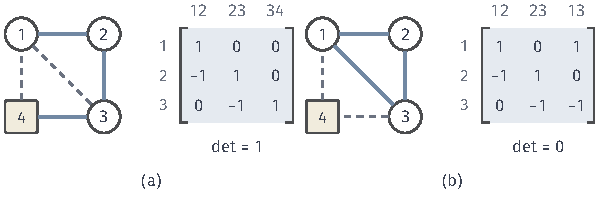
\includegraphics{figures/03-graphs/05-matrices-and-spectra/tikz/laplacian-tree-minors.pdf}
  \caption{固定根$4$后对照两组边的关联子式。方框标出根，它没有对应的矩阵行。实线表示选中的边，同时给出矩阵的列标。（a）生成树的子式行列式为一。（b）三角形的子式前两列相加等于第三列。}
  \label{fig:laplacian-tree-minors}
\end{BookInlineFigure}

\subsection{生成树的代数余子式计数}
\label{sec:graph-matrix-tree-proof}

现在把约化关联子式的判别性质与\BookChapterRef{chap:linear-operations}{卷二“向量、矩阵与张量的运算”章}的 Cauchy--Binet 公式结合起来，导出用拉普拉斯矩阵的代数余子式计数生成树的矩阵树定理。

从组合拉普拉斯矩阵$\bm L$中删去第$r$行和第$r$列，得到$(n-1)\times(n-1)$主子矩阵$\overline{\bm L}=\bm L^{(r,r)}$，其行列式$\det\overline{\bm L}=(-1)^{r+r}\det\bm L^{(r,r)}$正是对角位置$(r,r)$处的代数余子式$C_{r,r}$。

由关联分解式~\eqref{eq:graph-laplacian-incidence-factorization}，$\overline{\bm L}$的每个条目为
\[
  \overline L_{i,j}=\sum_{e\in E} B_{i,e}\,w_e\,B_{j,e},
\]
其中$i,j$遍历除$r$以外的$n-1$个顶点，求和仍遍及全部$m$条边。因此可以用$(n-1)\times m$约化关联矩阵$\overline{\bm B}$写成
\[
  \overline{\bm L}=\overline{\bm B}\,\bm C\,\overline{\bm B}^\top.
\]

进一步令$\bm M=\overline{\bm B}\bm C^{1/2}\in\mathbb R^{(n-1)\times m}$，使$\bm M$的每列为原来的约化关联列乘以该边权重的平方根$\sqrt{w_e}$。于是主子矩阵分解为
\[
  \overline{\bm L}=\bm M\bm M^\top,
\]
这正是 Cauchy--Binet 公式适用的矩形矩阵乘积形式。

\begin{theorem}[矩阵树定理]
\label{thm:graph-matrix-tree}
对有限无向非负权图，设$\mathcal T$为图的所有生成树的集合。则组合拉普拉斯矩阵$\bm L$在任意位置$(i,j)$处的代数余子式$C_{i,j}=(-1)^{i+j}\det\bm L^{(i,j)}$（特别地，删去任一顶点$r$的第$r$行与第$r$列所得的主余子式$\det\overline{\bm L}$）全部相等，且\term{矩阵树定理}（matrix-tree theorem）给出
\begin{equation}
  \det \overline{\bm L}=(-1)^{i+j}\det\bm L^{(i,j)}=\sum_{T\in\mathcal T}\prod_{e\in T}w_e.
  \label{eq:graph-matrix-tree}
\end{equation}
单位权时每棵生成树贡献$1$，该代数余子式就是生成树的数目。
\end{theorem}

\begin{proof}
第一步，对$(n-1)\times m$矩阵$\bm M$与$m\times(n-1)$矩阵$\bm M^\top$的乘积$\overline{\bm L}=\bm M\bm M^\top$应用 Cauchy--Binet 公式（参见\BookChapterRef{chap:linear-operations}{卷二“向量、矩阵与张量的运算”章}）。每次从$m$列中选出$n-1$个列指标（即选出一个$n-1$元边集$S\subseteq E$），由于$(\bm M^\top)_{S,:}=(\bm M_{:,S})^\top$，对应行和对应列组成的两个$(n-1)$阶子方阵互为转置、行列式相等，故
\[
  \det\overline{\bm L}
  =\sum_{\substack{S\subseteq E\\ |S|=n-1}}\det(\bm M_{:,S})\det\bigl((\bm M^\top)_{S,:}\bigr)
  =\sum_{\substack{S\subseteq E\\ |S|=n-1}}\det(\bm M_{:,S})^2.
\]

第二步，提取每条边的权重因子。$\bm M$的第$e$列是$\overline{\bm B}$的第$e$列乘以$\sqrt{w_e}$。取出$S$中各列后，由行列式对各列的齐次性，每列各提出一个$\sqrt{w_e}$因子，平方后变成$w_e$，因此
\[
  \det(\bm M_{:,S})^2=\det(\overline{\bm B}_{:,S})^2\prod_{e\in S}w_e.
\]

第三步，代入关联子式的判别结果。由引理~\ref{lem:graph-tree-incidence-minors}，如果$S$构成生成树，关联子式$\det(\overline{\bm B}_{:,S})$为$\pm1$，平方为$1$，该项贡献恰好是这棵生成树各边权重的乘积$\prod_{e\in S}w_e$；如果$S$不是生成树，关联子式为零，该项贡献为零。把所有非零项相加，即得对角位置的主余子式公式$\det\overline{\bm L}=\sum_{T\in\mathcal T}\prod_{e\in T}w_e$。

第四步，证明任意非对角位置$(i,j)$（$i\neq j$）的代数余子式$C_{i,j}=(-1)^{i+j}\det\bm L^{(i,j)}$也等于$\det\bm L^{(i,i)}$。在删去第$i$行与第$j$列所得的$(n-1)$阶子矩阵$\bm L^{(i,j)}$中，原矩阵的第$i$列保留了下来；将$\bm L^{(i,j)}$中除原第$i$列以外的其余$n-2$列全部加到原第$i$列上，行列式不变。由于$\bm L$的每一行元素之和为零（$\bm L\bm 1=\bm 0$），相加后原第$i$列在每一行上的新元素恰好等于$-\bm L^{(i,i)}$中原编号为$j$的列的元素。

最后，通过$|i-j|-1$次相邻列交换，把这一列移到原第$j$列在$\bm L^{(i,i)}$中的位置。列变号与列交换带来的总符号因子为$-(-1)^{|i-j|-1}=(-1)^{i+j}$，与代数余子式定义中的$(-1)^{i+j}$相乘恰好为$+1$，从而$(-1)^{i+j}\det\bm L^{(i,j)}=\det\bm L^{(i,i)}$。
\end{proof}

由于树权总和不涉及任何特定根，删去不同顶点的行列后得到的主余子式全都相等。含零权边的树在乘积中贡献为零；若正权支撑不连通，所有生成树至少包含一条零权边，权积全为零，代数余子式也为零。

下面在四点五边单位权算例上核对。删去顶点$3$对应的行和列，得到$3\times 3$约化矩阵
\[
  \overline{\bm L}=
  \begin{bmatrix}
  3&-1&-1\\
  -1&2&0\\
  -1&0&2
  \end{bmatrix}.
\]
沿第一行展开行列式：
\[
  \begin{aligned}
    \det\overline{\bm L}
    &=3\cdot\det\begin{bmatrix}2&0\\0&2\end{bmatrix}
      -(-1)\cdot\det\begin{bmatrix}-1&0\\-1&2\end{bmatrix}
      +(-1)\cdot\det\begin{bmatrix}-1&2\\-1&0\end{bmatrix}\\
    &=3\times 4 + 1\times(-2) - 1\times 2 = 12-2-2=8.
  \end{aligned}
\]

从组合计数看，五条边任选三条共有$\binom53=10$组。其中两个三角形$\{12,23,13\}$与$\{13,34,41\}$各自成环，贡献为零；其余$8$组各构成一棵生成树，单位权下各贡献$1$，总数为$8$。

若将对角边$13$的权重改为$2$，生成树的集合本身不变，但每棵包含边$13$的生成树权积变为$2$。含边$13$的生成树还需将顶点$2$和$4$分别接入$\{1,3\}$：顶点$2$可选边$12$或$23$（$2$种），顶点$4$可选边$34$或$41$（$2$种），共$2\times 2=4$棵。这$4$棵树各贡献$2$，其余$4$棵不含边$13$的树各贡献$1$，加权生成树总和变为$4\times 2+4\times 1=12$。

\subsection{生成树的拉普拉斯谱公式}
\label{sec:graph-tree-counting-formulas}

矩阵树定理把生成树权重总和表示为删去任一顶点行列所得的主余子式$\det\overline{\bm L}$。将全部$n$个顶点的主余子式汇总到$\bm L$的特征多项式一次项系数中，就可以直接用拉普拉斯矩阵的其余$n-1$个特征值$\lambda_2,\ldots,\lambda_n$表达生成树权重总和。

\begin{theorem}[生成树计数的拉普拉斯谱公式]
\label{cor:graph-tree-count-spectrum}
设$n\geq 2$，有限无向非负加权图的组合拉普拉斯特征值按升序排列为$0=\lambda_1\leq\lambda_2\leq\cdots\leq\lambda_n$。则图的生成树权重总和满足
\begin{equation}
  \sum_{T\in\mathcal T}\prod_{e\in T}w_e
  =\frac1n\prod_{i=2}^n\lambda_i.
  \label{eq:graph-tree-count-from-spectrum}
\end{equation}
\end{theorem}

\begin{proof}
第一步，从特征值展开计算$\det(t\bm I+\bm L)$中$t$的一次项系数。在$\bm L$的正交特征基下，$t\bm I+\bm L$的特征值为$t+\lambda_1,\ldots,t+\lambda_n$；因$\lambda_1=0$，有
\[
  \det(t\bm I+\bm L)=t\prod_{i=2}^n(t+\lambda_i).
\]
将其按$t$的幂展开，$t$的一次项系数为$\prod_{i=2}^n\lambda_i$。

第二步，从行列式按列的多线性计算同一系数。将$\det(t\bm I+\bm L)$的第$r$列写成$t\bm e_r + \bm L_{:,r}$；展开式中含$t$的一次项恰好来自“在某一列$r$选取$t\bm e_r$、在其余$n-1$列选取$\bm L$的原列”的所有组合。对固定的$r\in\{1,\ldots,n\}$，将第$r$列替换为$t\bm e_r$后沿第$r$列作拉普拉斯展开，所得$t$的系数正是删去$\bm L$的第$r$行与第$r$列后的主余子式$\det\overline{\bm L}^{(r)}$。

第三步，应用矩阵树定理求并比较系数。由定理~\ref{thm:graph-matrix-tree}，每个顶点$r$的主余子式均等于$\sum_{T\in\mathcal T}\prod_{e\in T}w_e$。对$r=1,\ldots,n$求和，可知$\det(t\bm I+\bm L)$中$t$的一次项系数又等于$n\sum_{T\in\mathcal T}\prod_{e\in T}w_e$。比较两种展开的一次项系数并除以$n$，即得式~\eqref{eq:graph-tree-count-from-spectrum}。
\end{proof}

在四点五边单位权算例中，第~\ref{sec:graph-laplacian-frequency}小节已算出$\bm L$的四个特征值为$0,2,4,4$。代入式~\eqref{eq:graph-tree-count-from-spectrum}得
\[
  \frac{1}{4}\times(2\times 4\times 4)=8,
\]
与上一小节直接展开$3\times 3$约化行列式所得的$8$棵生成树完全一致。

此外，若将全图所有边权同时乘以正数$a>0$，每棵生成树包含$n-1$条边，其边权乘积乘以$a^{n-1}$；与此同时，每个非零特征值$\lambda_i$也乘以$a$，式~\eqref{eq:graph-tree-count-from-spectrum}右侧$n-1$个特征值之积同样乘以$a^{n-1}$，两端具有相同的齐次尺度。

\subsection{完全图的Cayley公式}
\label{sec:graph-cayley-formula}

将第~\ref{sec:graph-typical-laplacian-spectra}小节求出的典型图拉普拉斯谱代入定理~\ref{cor:graph-tree-count-spectrum}，无需再逐个展开行列式，就能直接算出图族的生成树数目。其中最著名的应用是完全图$K_n$的生成树计数——由于$K_n$包含$n$个标号顶点之间的全部可能连边，$K_n$的生成树与$n$个标号顶点上的所有标号树一一对应。

\begin{theorem}[Cayley公式]
\label{thm:graph-cayley-formula}
设$n\geq 2$。单位权完全图$K_n$的生成树个数（即$n$个标号顶点上的标号树总数）满足\emph{Cayley公式}（Cayley's formula）：
\begin{equation}
  |\mathcal T(K_n)|=n^{n-2}.
  \label{eq:graph-cayley-count}
\end{equation}
\end{theorem}

\begin{proof}
由定理~\ref{prop:graph-typical-laplacian-spectra}，单位权完全图$K_n$的组合拉普拉斯谱为$\lambda_1=0$（重数$1$）与$\lambda_2=\cdots=\lambda_n=n$（重数$n-1$）。代入谱公式~\eqref{eq:graph-tree-count-from-spectrum}，立得
\[
  |\mathcal T(K_n)|=\frac{1}{n}\prod_{i=2}^n n=\frac{1}{n}\cdot n^{n-1}=n^{n-2}.
\]
\end{proof}

也可以直接在约化矩阵上核对完全图的 Cayley 公式：从$\bm L(K_n)=n\bm I_n-\bm 1_n\bm 1_n^\top$中删去一行一列后，$(n-1)\times(n-1)$约化矩阵为$\overline{\bm L}=n\bm I_{n-1}-\bm 1_{n-1}\bm 1_{n-1}^\top$。该矩阵在全一向量$\bm 1_{n-1}$方向上的特征值为$n-(n-1)=1$，在正交补上的$n-2$个特征值仍为$n$，特征值乘积同样给出$\det\overline{\bm L}=1\cdot n^{n-2}=n^{n-2}$。

用同样的方法核对星图$K_{1,n-1}$：由定理~\ref{thm:graph-star-laplacian-spectrum}知其非零拉普拉斯特征值为$n-2$个$1$和$1$个$n$，代入式~\eqref{eq:graph-tree-count-from-spectrum}得$|\mathcal T(K_{1,n-1})|=\frac{1}{n}(1^{n-2}\cdot n)=1$，与树本身只有唯一一棵生成树一致。

\section{归一化拉普拉斯}
\label{sec:graph-normalized-laplacian}

前面几节讨论的组合拉普拉斯矩阵$\bm L=\bm D-\bm W$在标准欧氏内积下给每个顶点相同的单位权重$1$。它可描述以边权为跳转速率的连续时间扩散；若采用每步跳转一次、按边权比例选择邻居的离散随机游走，则应使用按度归一化的算子。两种模型的时间尺度不同。下面通过两个例子说明归一化的作用（图~\ref{fig:laplacian-diffusion-bottleneck}）。

第一个例子是图~\ref{fig:laplacian-diffusion-bottleneck}(a)所示的“双团哑铃图”：两个各含$m$个顶点的稠密完全图团$K_m$之间仅通过一条单位权桥边$u\!-\!v$相连。在桥端点$u$处，共有$m-1$条边连向同侧团内部，只有$1$条桥边连向对侧团（度数为$d_u=m$）。当一个随机游走粒子到达$u$时，它在下一步等概率地从$m$条关联边中任选一条迈出，因此只有$\frac{1}{m}$的概率跨过桥边进入右侧团，而有$\frac{m-1}{m}$的概率退回左侧团内部。当团规模$m$很大时，尽管桥边的绝对权重仍为$1$，粒子在桥端点跨团转移的概率却因团内邻接边增多而降为$\frac{1}{m}$，全图的跨团混合速度随团规模增大而变慢。

第二个例子是图~\ref{fig:laplacian-diffusion-bottleneck}(b)所示的含高连接度枢纽的网络：中心枢纽顶点$h$连接了$D\gg 1$条边，而右侧普通顶点$i$只连接$2$条边。粒子从普通顶点$i$出发时，每条关联边分到$\frac{1}{2}$的转移概率；而从枢纽顶点$h$出发时，每条边分到的转移概率$w_{h,j}/d_h$为$\frac{1}{D}$。

若把全图所有边权同时乘以$10$，每个正度顶点按权重比例选择邻居的转移概率$w_{i,j}/d_i$保持不变，离散随机游走也保持不变；组合拉普拉斯及其特征值则乘以$10$，对应连续时间扩散加速$10$倍。若只缩放局部边权，边界顶点的转移概率一般会改变，不能作相同推断。

\begin{BookInlineFigure}
  \centering
  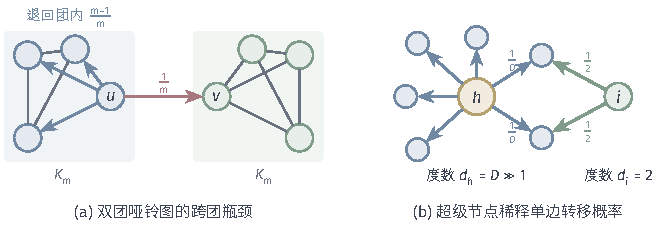
\includegraphics[width=111.633mm]{figures/03-graphs/05-matrices-and-spectra/tikz/laplacian-diffusion-bottleneck/figure.pdf}
  \caption{度数分布对一步随机游走转移概率的稀释效应。（a）双团哑铃图中，桥端点$u$有$m-1$条团内边和$1$条跨团桥边，粒子跨过桥边的概率仅为$1/m$，以$(m-1)/m$的概率退回原团。（b）度数为$D\gg 1$的枢纽顶点$h$将每条关联边上的转移概率稀释为$1/D$，而度数为$2$的普通节点$i$在每条边上分配$1/2$的转移概率。}
  \label{fig:laplacian-diffusion-bottleneck}
\end{BookInlineFigure}

在每步跳转一次的离散随机游走模型中，转移概率取决于边权占顶点加权度的比例，跨区瓶颈则与割权占集合体积$\operatorname{vol}(S)=\sum_{i\in S}d_i$的比例有关。归一化谱与这一时间尺度相适应。

为研究上述离散随机游走，使用度矩阵$\bm D$对拉普拉斯矩阵作归一化。本节先引入以度数计权的度加权内积与集合体积，再分别构造对称归一化拉普拉斯$\mathcal L=\bm D^{-1/2}\bm L\bm D^{-1/2}$和随机游走拉普拉斯$\bm L_{\mathrm{rw}}=\bm D^{-1}\bm L$，对比两种归一化算子的联系与分工，最后证明归一化拉普拉斯谱的性质。

\subsection{度加权内积}
\label{sec:graph-degree-weighted-inner-product}

标准欧氏长度平方$\sum_i x_i^2$给每个顶点相同的权重$1$。为了按每个顶点的连接量计权，将第$i$个坐标的权重替换为该顶点的加权度$d_i$，在正度顶点集$V_+=\{i\in V:d_i>0\}$上定义\term{度加权内积}（degree-weighted inner product）及其诱导范数：
\begin{equation}
  \langle \bm x,\bm y\rangle_{\bm D}
  =\bm x^\top\bm D\bm y
  =\sum_{i\in V_+}d_i\,x_iy_i,
  \qquad
  \lVert\bm x\rVert_{\bm D}^2=\bm x^\top\bm D\bm x.
  \label{eq:graph-degree-weighted-inner-product}
\end{equation}
在$V_+$上所有$d_i>0$，故任意非零向量的度加权长度平方$\lVert\bm x\rVert_{\bm D}^2>0$，式~\eqref{eq:graph-degree-weighted-inner-product}确实构成$V_+$上的内积。

用度加权范数衡量单点脉冲$\bm e_i$（$i\in V_+$）时，其沿边变化能量为$\bm e_i^\top\bm L\bm e_i=d_i$，度加权长度平方同样为$\lVert\bm e_i\rVert_{\bm D}^2=d_i$，两者之比对任意正度顶点都恒等于
\[
  \frac{\bm e_i^\top\bm L\bm e_i}{\lVert\bm e_i\rVert_{\bm D}^2}=\frac{d_i}{d_i}=1.
\]
例如在四点五边单位权图上，度为$3$的顶点$1$与度为$2$的顶点$2$在标准欧氏范数下的单位脉冲能量分别为$3$和$2$，而在度加权范数下，每单位连接量所承担的变化比值完全一致，均为$1$。

将任意顶点子集$S\subseteq V$的指示向量$\bm 1_S$代入度加权长度平方，立得子集内各顶点的加权度总和：
\begin{equation}
  \operatorname{vol}(S)=\sum_{i\in S}d_i
  =\lVert\bm1_S\rVert_{\bm D}^2.
  \label{eq:graph-laplacian-vertex-volume}
\end{equation}
这个和称为顶点子集$S$的\emph{体积}（volume），它精确计量了$S$所关联的边权容量：两端都在$S$内部的边在两个端点各计一次共两倍权重，跨出$S$的边计一倍权重。例如四点五边图中$S=\{1,2\}$的体积为$d_1+d_2=3+2=5$。

结合第~\ref{sec:graph-laplacian-energy}节的割权公式$\bm 1_S^\top\bm L\bm 1_S=c(S,V\setminus S)$，指示向量$\bm 1_S$的度加权Rayleigh商为
\[
  \frac{\bm 1_S^\top\bm L\bm 1_S}{\bm 1_S^\top\bm D\bm 1_S}
  =\frac{c(S,V\setminus S)}{\operatorname{vol}(S)}.
\]
这一比值直接给出了切开$S$的跨割边权重占$S$总连接体积的比例——这正是第~\ref{chap:spectral-partition}章导通率与归一化割（NCut）的核心度量。

需要注意，孤立顶点的加权度$d_i=0$，一个只在孤点上取$1$的非零向量在$\bm x^\top\bm D\bm x$下得零值，因此在包含孤点的全空间上$\sqrt{\bm x^\top\bm D\bm x}$只是半范数，相应双线性型不构成正定内积。下面的推导先在正度顶点集$V_+$上进行，再约定孤点在全空间矩阵中的零扩展。

\subsection{对称归一化拉普拉斯}
\label{sec:graph-symmetric-normalized-laplacian}

在$V_+$上，一组读数的能量与度加权长度平方之比为
\[
  \frac{\bm x^\top\bm L\bm x}{\bm x^\top\bm D\bm x},
  \qquad \bm x\ne\bm0.
\]
这是一个广义 Rayleigh 商。如果能把分母变成普通欧氏长度平方，就可以直接使用对称矩阵的谱分析工具。

观察分母中的每一项$d_ix_i^2$。它可以写成$(\sqrt{d_i}\,x_i)^2$。这就提示我们引入新坐标$y_i=\sqrt{d_i}\,x_i$。在正度顶点上，这个变换是可逆的：$x_i=y_i/\sqrt{d_i}$。新坐标描述的仍然是同一组读数，只是数值按度的平方根缩放了。

以四点图上的常值读数$x_i=1$为例。顶点$1$和$3$的度为$3$，对应新坐标为$\sqrt3$。顶点$2$和$4$的度为$2$，对应新坐标为$\sqrt2$。尽管四个新坐标的数值不同，还原后的实际读数仍然处处相等。

将$\bm x=\bm D^{-1/2}\bm y$代入分子，左右各出现一个$\bm D^{-1/2}$：
\[
  \bm x^\top\bm L\bm x
  =\bm y^\top(\bm D^{-1/2}\bm L\bm D^{-1/2})\bm y.
\]
分母已经变成$\bm y^\top\bm y$。整个比值成为新坐标上一个对称矩阵的普通 Rayleigh 商。矩阵极值性质可参考\BookChapterRef{chap:matrix-approximation}{卷二"矩阵逼近"章}。

\begin{definition}[对称归一化拉普拉斯]
\label{def:graph-symmetric-normalized-laplacian}
在正度顶点上，\term{对称归一化拉普拉斯}（symmetric normalized Laplacian）定义为
\begin{equation}
  \begin{aligned}
  \mathcal L&=\bm D^{-1/2}\bm L\bm D^{-1/2}\\
            &=\bm I-\bm D^{-1/2}\bm W\bm D^{-1/2}.
  \end{aligned}
  \label{eq:graph-symmetric-normalized-laplacian}
\end{equation}
含孤点时，在$\bm D^{-1/2}$中将孤点位置取零，用第一式定义全空间上的矩阵。
\end{definition}

在新坐标中，一条边比较的是$y_i/\sqrt{d_i}$和$y_j/\sqrt{d_j}$，即还原后的实际读数。因此，原读数在某个连通分量上取常值$1$、分量外取$0$时，新坐标中的零方向变为$\bm D^{1/2}\bm1_{V_a}$，即各点取$\sqrt{d_i}$。图~\ref{fig:laplacian-degree-coordinates}展示了四点图上常值读数的两种坐标。右图中四个坐标因度而异，但还原为实际读数后各边差值仍为零。

\begin{BookInlineFigure}
  \centering
  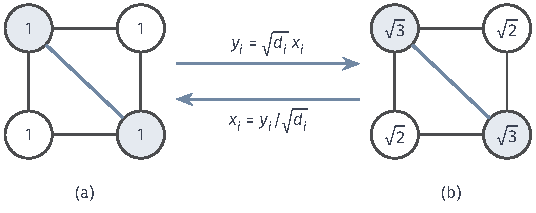
\includegraphics{figures/03-graphs/05-matrices-and-spectra/tikz/laplacian-degree-coordinates.pdf}
  \caption{同一组常值读数的两种坐标。浅蓝顶点度为三，白色顶点度为二。（a）原读数都为一。（b）按度的平方根缩放后，坐标因度而异。计算边差时，先按下方箭头把每个坐标还原。}
  \label{fig:laplacian-degree-coordinates}
\end{BookInlineFigure}

现在把孤点放回全空间。规定孤点在矩阵中有一行零、一列零，表示它的读数不参与任何邻居的计算。$\bm D^{-1/2}$在全空间中的对角矩阵于是在孤点位置取零。坐标的可逆换元仍然只在正度空间上使用。

如果按式~\eqref{eq:graph-symmetric-normalized-laplacian}的第二行来理解全空间矩阵，就需要注意单位阵的对应调整。在第一行中，$\bm D^{-1/2}\bm D\bm D^{-1/2}$在正度位置得到$1$，在孤点位置得到$0$。因此第二行的$\bm I$应当理解为$\bm\Pi_+$，即正度处取$1$、孤点处取$0$的对角投影阵。

用一个小例子核验。只在顶点$1,2$之间放一条单位权边，顶点$3$为孤点。$\bm D=\operatorname{diag}(1,1,0)$，按定义得到
\[
  \mathcal L=\begin{bmatrix}1&-1&0\\-1&1&0\\0&0&0\end{bmatrix}.
\]
零空间由$(1,1,0)^\top$和$(0,0,1)^\top$张成。如果错把孤点的对角元设成$1$，就会丢掉孤点对应的零方向。

\subsection{随机游走拉普拉斯}
\label{sec:graph-random-walk-laplacian}

归一化邻居平均提供了第二种视角。对正度顶点$i\in V_+$，将每个邻居的边权除以该点的总加权度$d_i$，所得$P_{i,j}=w_{i,j}/d_i$是邻居$j$在顶点$i$的所有连接中所占的权重份额。所有份额非负且总和为$\sum_j P_{i,j}=1$，因此
\begin{equation}
  (\bm P\bm x)_i=\sum_{j=1}^n\frac{w_{i,j}}{d_i}x_j
  \label{eq:graph-random-walk-neighbor-average}
\end{equation}
正是顶点$i$的邻居读数的加权平均。若某个顶点$i$是零度孤点（$d_i=0$），约定其保持原读数不变，即令$P_{i,i}=1$且$P_{i,j}=0$（$j\ne i$）。

\begin{definition}[随机游走拉普拉斯]
\label{def:graph-random-walk-laplacian}
设$\bm P$为按上述规则定义的邻域平均矩阵。图的\term{随机游走拉普拉斯}（random-walk Laplacian）定义为
\begin{equation}
  \bm L_{\mathrm{rw}}=\bm I-\bm P.
  \label{eq:graph-random-walk-laplacian}
\end{equation}
在正度顶点集$V_+$上，$\bm P=\bm D^{-1}\bm W$，从而$\bm L_{\mathrm{rw}}=\bm I-\bm D^{-1}\bm W=\bm D^{-1}\bm L$。
\end{definition}

随机游走拉普拉斯直接以原顶点读数$\bm x$为输入，在每个正度顶点$i$处输出本点读数$x_i$减去邻居加权平均$(\bm P\bm x)_i$的偏离量；在孤点处，因$(\bm P\bm x)_i=x_i$，输出恒为零。

在四点五边单位权图上取$\bm x=(1,0,1,0)^\top$核对：组合拉普拉斯输出为$\bm L\bm x=(2,-2,2,-2)^\top$，逐行除以各点度数$(3,2,3,2)$即得
\[
  \bm L_{\mathrm{rw}}\bm x=(2/3,-1,2/3,-1)^\top.
\]
逐点检查：顶点$1$的三个邻居$2,3,4$读数为$0,1,0$，平均值为$1/3$，本点读数$1$减去$1/3$得$2/3$；顶点$2$的两个邻居$1,3$读数均为$1$，平均值为$1$，本点读数$0$减去$1$得$-1$。

虽然在度数不均匀的图上，$\bm P=\bm D^{-1}\bm W$与$\bm L_{\mathrm{rw}}=\bm D^{-1}\bm L$在标准欧氏内积下一般不对称，但在正度空间$V_+$的度加权内积$\langle\cdot,\cdot\rangle_{\bm D}$下，它们都是自伴算子。事实上，由$\bm D\bm P=\bm W=\bm W^\top=\bm P^\top\bm D$，对任意$\bm x,\bm y\in\mathbb R^{V_+}$有
\[
  \begin{aligned}
    \langle \bm x,\bm P\bm y\rangle_{\bm D}
    &=\bm x^\top\bm D\bm P\bm y\\
    &=\bm x^\top\bm W\bm y\\
    &=(\bm P\bm x)^\top\bm D\bm y
     =\langle \bm P\bm x,\bm y\rangle_{\bm D}.
  \end{aligned}
\]

名称中的“随机游走”源于$P_{i,j}=w_{i,j}/d_i$的概率解释：将其视为从顶点$i$出发下一步随机移向邻居$j$的转移概率时，$(\bm P\bm x)_i$恰好是下一步所在顶点读数的条件期望。第~\ref{chap:graph-walks}章将围绕转移矩阵$\bm P$展开图上随机游走的分布演化与收敛分析。

\subsection{两种归一化拉普拉斯的对比}
\label{sec:graph-normalized-laplacian-comparison}

对称归一化拉普拉斯$\mathcal L=\bm D^{-1/2}\bm L\bm D^{-1/2}$与随机游走拉普拉斯$\bm L_{\mathrm{rw}}=\bm D^{-1}\bm L=\bm I-\bm P$从不同方式对度数作了归一化，二者在相似关系、对称性与应用场景上既有紧密联系，又有明确分工。

\paragraph{相似关系}
在正度空间$V_+$上，先用$\bm D^{-1/2}$把缩放坐标还原为原顶点读数，再作用$\bm L_{\mathrm{rw}}=\bm D^{-1}\bm L$，最后用$\bm D^{1/2}$转回缩放坐标，合并左侧的$\bm D^{1/2}\bm D^{-1}=\bm D^{-1/2}$即得相似恒等式
\begin{equation}
  \mathcal L=\bm D^{-1/2}\bm L\bm D^{-1/2}=\bm D^{1/2}\bm L_{\mathrm{rw}}\bm D^{-1/2}.
  \label{eq:graph-normalized-laplacian-similarity}
\end{equation}
因此，$\mathcal L$与$\bm L_{\mathrm{rw}}$在$V_+$上互为相似矩阵，拥有完全相同的特征值（连同每个零度孤点在两个矩阵中各自贡献的一个零特征值，两者在全空间上的谱也完全一致）。

两者的特征向量之间相差一个度平方根缩放因子：若$\bm x\in\mathbb R^{V_+}$满足$\bm L_{\mathrm{rw}}\bm x=\mu\bm x$，左乘$\bm D^{1/2}$即知$\bm y=\bm D^{1/2}\bm x$满足$\mathcal L\bm y=\mu\bm y$。特别地，对于零特征值$\mu=0$，$\bm L_{\mathrm{rw}}$在连通分量上的零特征向量是处处相等的常值向量$\bm 1_{V_a}$，而$\mathcal L$对应的零特征向量则是按度平方根加权的$\bm D^{1/2}\bm 1_{V_a}$。

\paragraph{对称性}
$\mathcal L$从左右两侧对称地乘上$\bm D^{-1/2}$，在标准欧氏内积$\langle\bm y,\bm y'\rangle=\bm y^\top\bm y'$下是实对称矩阵（$\mathcal L^\top=\mathcal L$），其不同特征子空间关于标准欧氏内积正交。

$\bm L_{\mathrm{rw}}=\bm D^{-1}\bm L$只在左侧乘以$\bm D^{-1}$，一般不对称；只有每条正权边的两端加权度相等时才对称（不同连通分量可以有不同的度）；但它在度加权内积$\langle\bm x,\bm x'\rangle_{\bm D}=\bm x^\top\bm D\bm x'$下自伴，可选取关于度加权内积$\bm D$-正交的特征向量基，这恰好对应缩放后的向量$\bm y=\bm D^{1/2}\bm x$关于标准欧氏内积正交。

\paragraph{应用场景}
当需要利用实对称矩阵的正交谱分解、Courant--Fischer极小极大原理或矩阵范数工具（例如第~\ref{chap:spectral-partition}章求解归一化割NCut的谱松弛与第~\ref{chap:graph-sparsification}章的谱稀疏化）时，采用实对称的$\mathcal L$最为直接。

当需要直接对原顶点函数作局部邻域加权平均、或追踪概率分布在图上一步步扩散的马尔可夫链演化（例如第~\ref{chap:graph-walks}章的随机游走与PageRank）时，采用保持行和为零的$\bm L_{\mathrm{rw}}=\bm I-\bm P$更为自然。当图为正度$d$正则图时，$\bm D=d\bm I$，两种归一化矩阵合二为一，均简化为$\mathcal L=\bm L_{\mathrm{rw}}=\bm L/d$。

\subsection{归一化拉普拉斯谱的性质}
\label{sec:graph-normalized-laplacian-spectrum}

由于$\mathcal L$与$\bm L_{\mathrm{rw}}$具有相同的特征值，我们统称其为图的\emph{归一化拉普拉斯谱}。下面的定理证明，按度归一化后，任意图的全部特征值都被收束在无量纲的固定区间$[0,2]$内，且上界$\mu=2$直接刻画了图的二部性。

\begin{theorem}[归一化拉普拉斯谱的范围]
\label{prop:graph-normalized-spectrum-bound}
有限无向非负加权图的对称归一化拉普拉斯$\mathcal L$（以及随机游走拉普拉斯$\bm L_{\mathrm{rw}}$）的全部特征值$\mu$均满足
\begin{equation}
  0\leq\mu\leq2.
  \label{eq:graph-normalized-spectrum-bound}
\end{equation}
其中零特征值的重数等于正权支撑$\mathcal G_+$的连通分量个数$c$；最大特征值达到上界$\mu=2$当且仅当正权支撑$\mathcal G_+$至少含有一个带正权边的二部连通分量。
\end{theorem}

\begin{proof}
第一步，将特征值写为度加权Rayleigh商并确定下界与零特征值重数。孤立顶点在$\mathcal L$和$\bm L_{\mathrm{rw}}$上均对应零特征值且自成无边的连通分量，故只需在正度顶点集$V_+$上分析。设非零向量$\bm x\in\mathbb R^{V_+}$满足$\bm L_{\mathrm{rw}}\bm x=\mu\bm x$，即$\bm D^{-1}\bm L\bm x=\mu\bm x$。左乘$\bm x^\top\bm D$并除以$\bm x^\top\bm D\bm x>0$，得
\[
  \mu=\frac{\bm x^\top\bm L\bm x}{\bm x^\top\bm D\bm x}
  =\frac{\sum_{\{i,j\}\in E}w_{i,j}(x_i-x_j)^2}{\sum_{i\in V_+}d_i x_i^2}.
\]
分子非负给出$\mu\geq 0$；且$\mu=0\iff\bm x^\top\bm L\bm x=0$，由定理~\ref{thm:graph-laplacian-components}知这等价于$\bm x$在每个正权连通分量上取常值，连同孤点在内零特征值重数恰为$c$。

第二步，证明上界$\mu\leq 2$。将$2\bm x^\top\bm D\bm x=2\sum_{i\in V_+}d_i x_i^2=\sum_{\{i,j\}\in E}2w_{i,j}(x_i^2+x_j^2)$与分子$\bm x^\top\bm L\bm x=\sum_{\{i,j\}\in E}w_{i,j}(x_i-x_j)^2$作差，利用代数恒等式$2(x_i^2+x_j^2)-(x_i-x_j)^2=(x_i+x_j)^2$，得到
\[
  2\bm x^\top\bm D\bm x-\bm x^\top\bm L\bm x
  =\sum_{\{i,j\}\in E}w_{i,j}(x_i+x_j)^2\geq 0.
\]
两端除以$\bm x^\top\bm D\bm x>0$即得$2-\mu\geq 0$，即$\mu\leq 2$。

第三步，分析取等号$\mu=2$的充要条件。上式取等号当且仅当存在非零向量$\bm x\in\mathbb R^{V_+}$使得$\sum_{\{i,j\}\in E}w_{i,j}(x_i+x_j)^2=0$，即对每条正权边$\{i,j\}\in E_+$都有$x_i+x_j=0$（$x_j=-x_i$）。

若$\mu=2$，任取$\bm x$的一个非零分量顶点$u\in V_+$，其所在正权连通分量$C$至少含有一条正权边。沿$C$中的任意正权路径每走一步，顶点读数变为相反数，故$C$中所有顶点的读数均取$\pm|x_u|\neq 0$，且每条正权边都连接一个取$+|x_u|$的顶点和一个取$-|x_u|$的顶点；将$C$按读数的正负号划分为两部分，即知$C$为含边的二部连通分量。

反之，若$\mathcal G_+$含有一个带边的二部连通分量$C=A\cup B$，令$\bm x$在$A$上取$+1$、在$B$上取$-1$、在其余分量上取$0$，则$\bm x\in\mathbb R^{V_+}$非零且在每条正权边上满足$x_i+x_j=0$，其度加权Rayleigh商达到$\mu=2$。
\end{proof}

这一结论可与第~\ref{sec:adjacency-bipartite-symmetry}小节二部图邻接谱的对称性对照：在四点单位权图上，四元环$C_4$是二部图，沿环交替赋$+1,-1$即可使每条边两端互为相反数，达到$\mu=2$；添入对角边$13$后，顶点$1$和$3$被连入同一个三角形，无法再为三个两两相邻的顶点同时赋予互为相反数的非零值，故四点五边图的归一化拉普拉斯最大特征值严格小于$2$。

最后考察边权整体缩放：若将全图所有边权同时乘以正数$a>0$，则$\bm L$和$\bm D$同时乘以$a$，$\mathcal L=\bm D^{-1/2}\bm L\bm D^{-1/2}$中两侧的$a^{-1/2}$与中间的$a$恰好抵消，随机游走矩阵$\bm P=\bm D^{-1}\bm W$也保持不变，说明归一化谱完全消除了边权的整体量纲尺度。例如四元环$C_4$的组合拉普拉斯谱为$0,2,2,4$，除以正则度数$d=2$即得归一化谱$0,1,1,2$，无论把四条边的权重同时改为何种正数，这一归一化谱始终不变。

\section{本章小结}
\label{sec:graph-laplacian-summary}

组合拉普拉斯把沿边取差、乘权和返回顶点三个步骤合成为$\bm L=\bm B\bm C\bm B^\top$。逐点来看，它输出的是每个顶点与邻居的带权偏离之和。若要衡量整张图上读数的变化而不让正负相消，就逐边取差、平方、乘权再求和。这个沿边变化能量恰好等于拉普拉斯的二次型$\bm x^\top\bm L\bm x$。

能量为零要求每条正权边的两端读数相等。沿正权路径传递这个等值关系，每个连通分量上的读数各为常值，分量之间可以独立选择。分量的个数就是零特征值的重数。

按边集展开约化拉普拉斯的行列式时，只有构成生成树的边组留下非零的关联子式。因此，删去任一个顶点对应的行和列后所得的主余子式都给出同一个树权总和。对正权支撑连通的图，也可以用$n-1$个非零特征值的乘积除以顶点数$n$来计算它。

每个特征值还描述了对应单位特征向量的变化尺度——长度为一的读数方向上的沿边能量。加边使每个方向的单位能量不减，进而使按大小排序的各特征值逐个不减。

三种矩阵使用不同的内积和坐标。组合拉普拉斯$\bm L=\bm D-\bm W$在原顶点读数上计算带权差的总和。随机游走拉普拉斯$\bm L_{\mathrm{rw}}=\bm I-\bm P$用同样的原顶点读数，输出的是本点读数与邻居加权平均的差。对称归一化拉普拉斯$\mathcal L=\bm D^{-1/2}\bm L\bm D^{-1/2}$在缩放坐标$\bm y=\bm D^{1/2}\bm x$上计算，使得度加权能量比变成普通 Rayleigh 商。三种形式的零方向都来自各分量上的常值读数——在原坐标中是分量指示向量$\bm1_{V_a}$，在缩放坐标中变为$\bm D^{1/2}\bm1_{V_a}$。三种矩阵都对孤点留出零块。

后续各章使用的矩阵形式各不相同。第~\ref{chap:graph-electrical-networks}章的电网络从注入电流出发求电势，方程的系数是组合拉普拉斯。第~\ref{chap:spectral-partition}章要比较连接量不同的顶点集合两侧的割与体积，归一化形式提供了按体积计量的尺度。第~\ref{chap:graph-walks}章用转移矩阵$\bm P$描述逐步选择邻居的演化，从邻居平均出发的收敛分析建立在归一化谱之上。

